\chapter{Methodology}
\label{cp:methodology}
\section{Apparatus} \label{sec:Apparatus}
A \acrshort{piv} system is set up to view flow over an airfoil in a wind tunnel. This system begins with putting an airfoil in a wind tunnel, as shown in \autoref{fig:test_section}. \autoref{fig:laser} shows the laser used in this lab, which is reflected off a mirror to illuminate particles in the flow. A smoke machine, such as the one in \autoref{fig:smoke_machine}, is also used to make the particles easier to identify and track. To record data, a high speed camera is used for image acquisition. To control the timing of the camera's photos and the laser illumination, a digital delay generator is used. The camera used can be seen in \autoref{fig:high-speed_camera}, and the digital delay generator can be seen in \autoref{fig:delay_generator}. The camera images are collected using data acquisition software on a computer. \autoref{fig:full_apparatus} depicts the full \acrshort{piv} system ready for operation.

\begin{figure}[htpb]
    \centering
    \begin{subfigure}{0.49\textwidth}
        \centering
        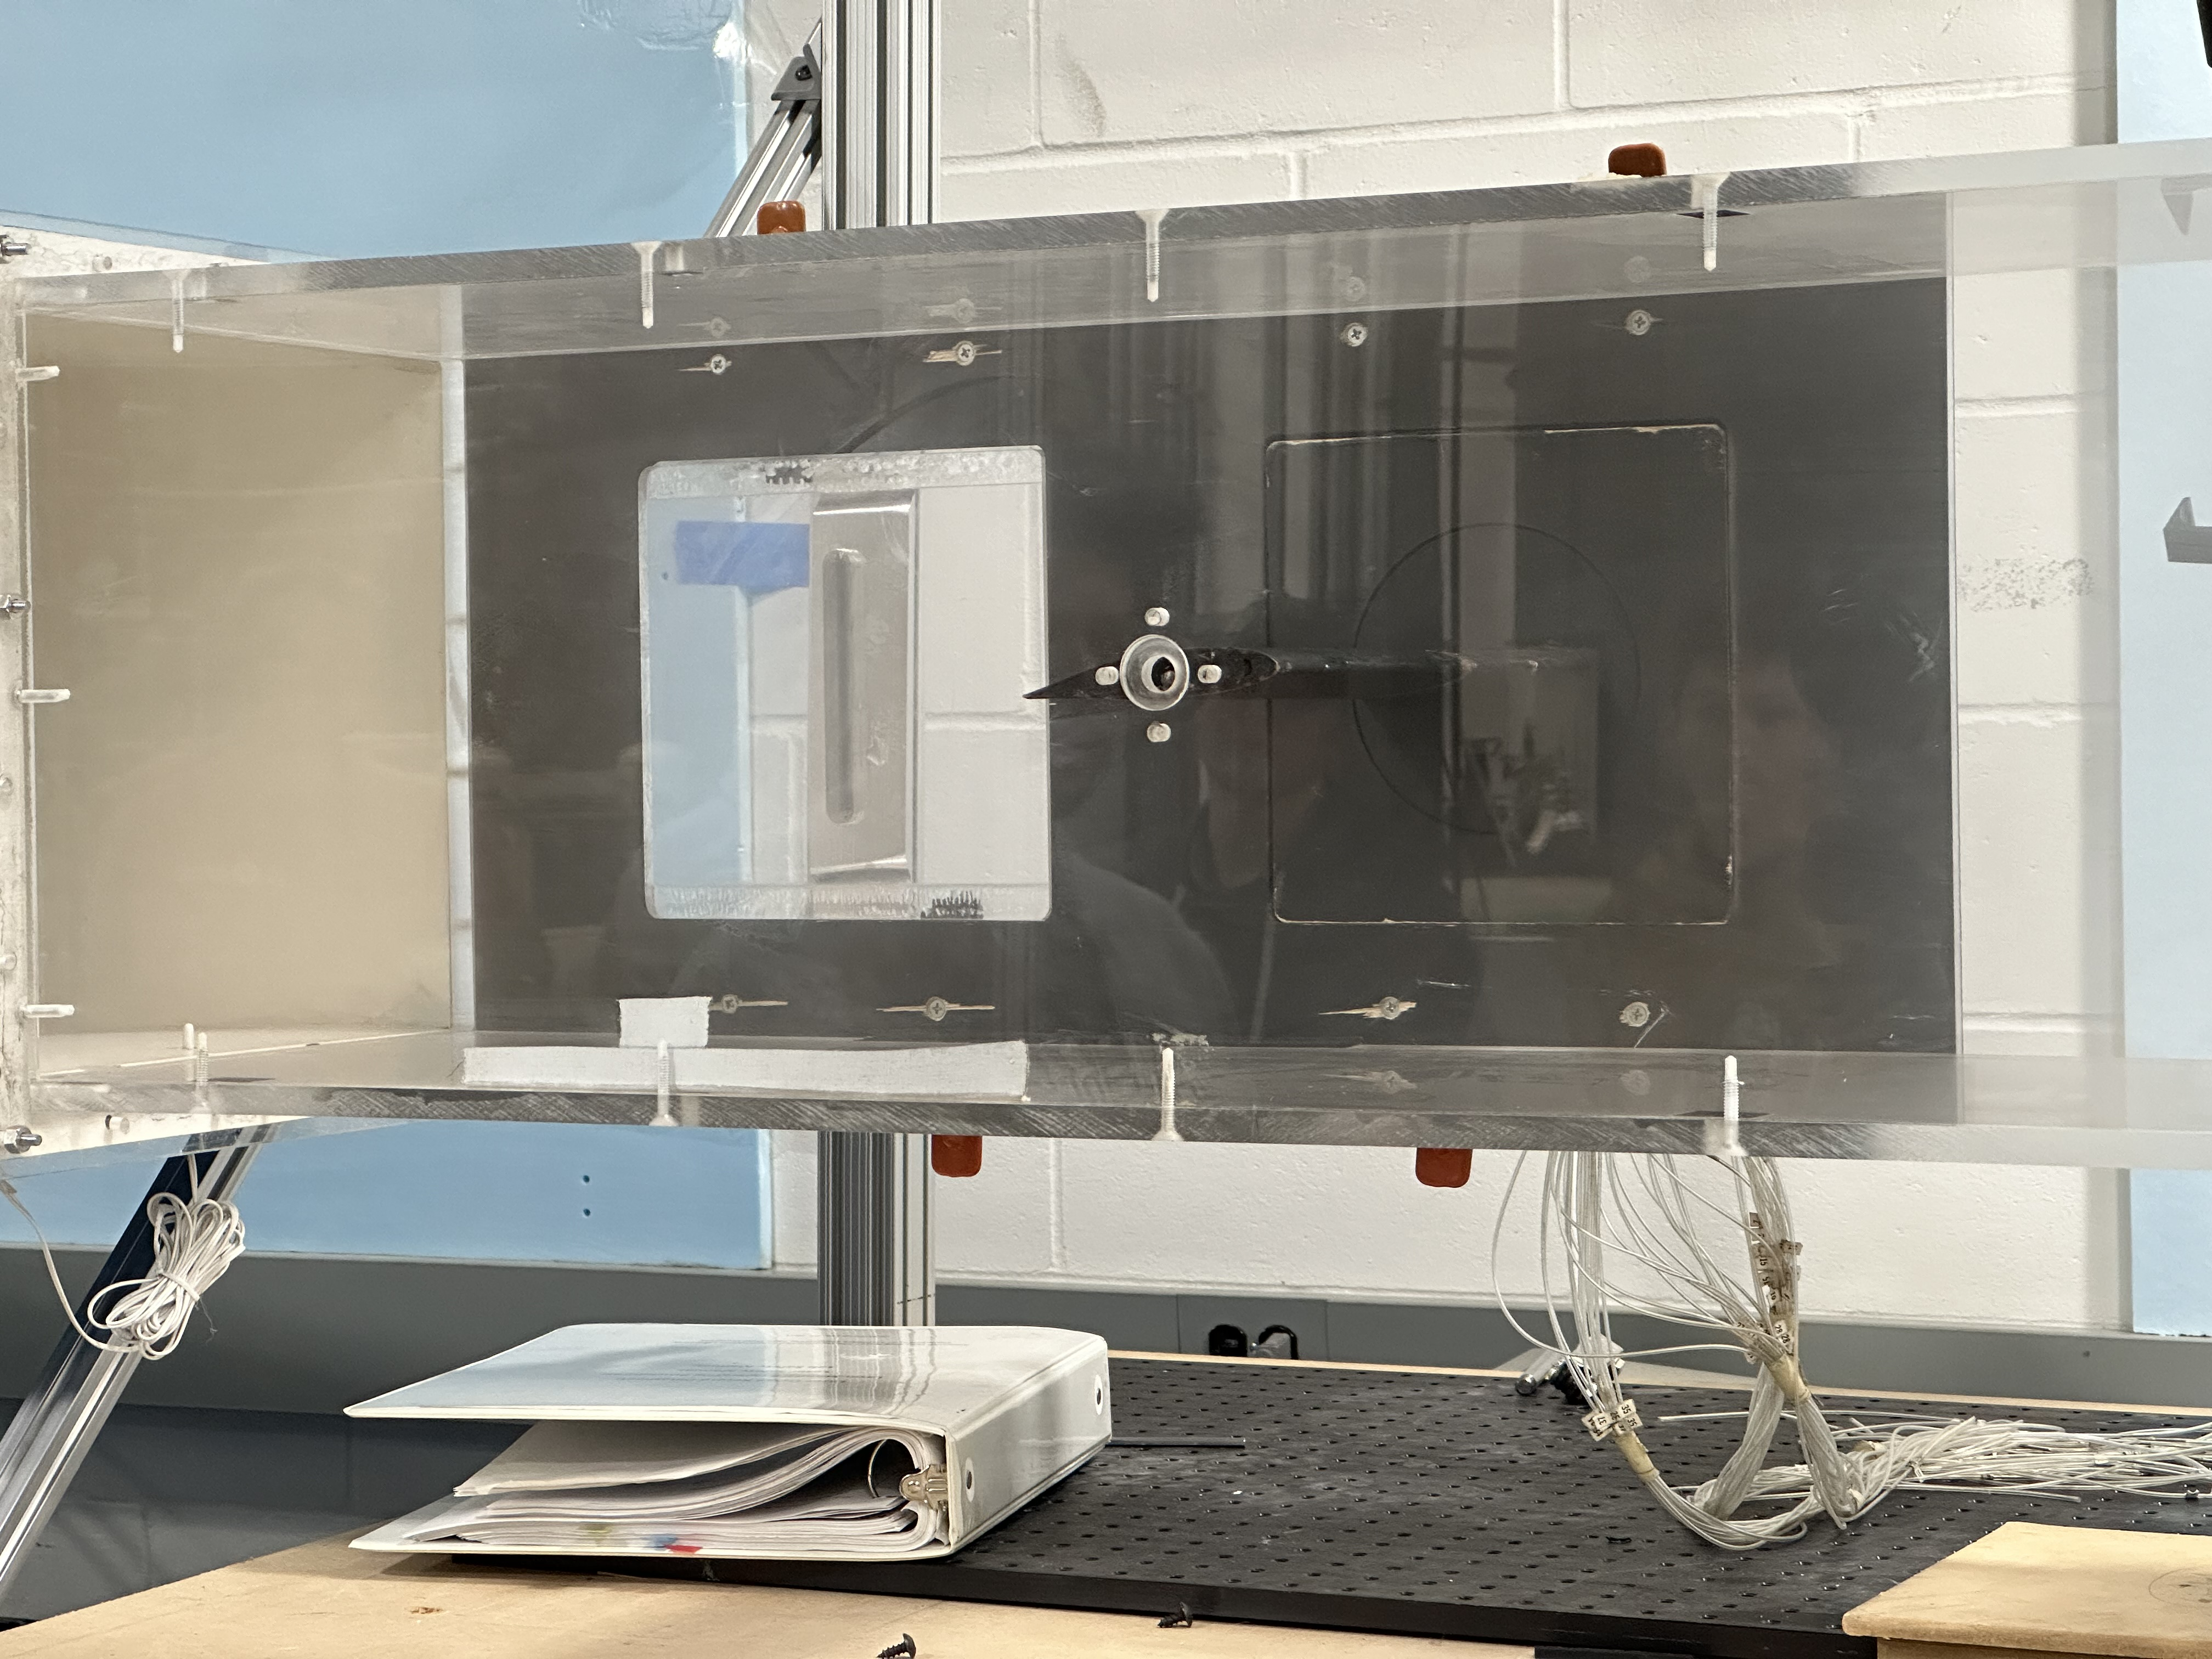
\includegraphics[width=\textwidth]{Figures/IMG_0127.jpeg}
        \caption{An airfoil inside the wind tunnel test section.}
        \label{fig:test_section}
    \end{subfigure}
    \begin{subfigure}{0.49\textwidth}
        \centering
        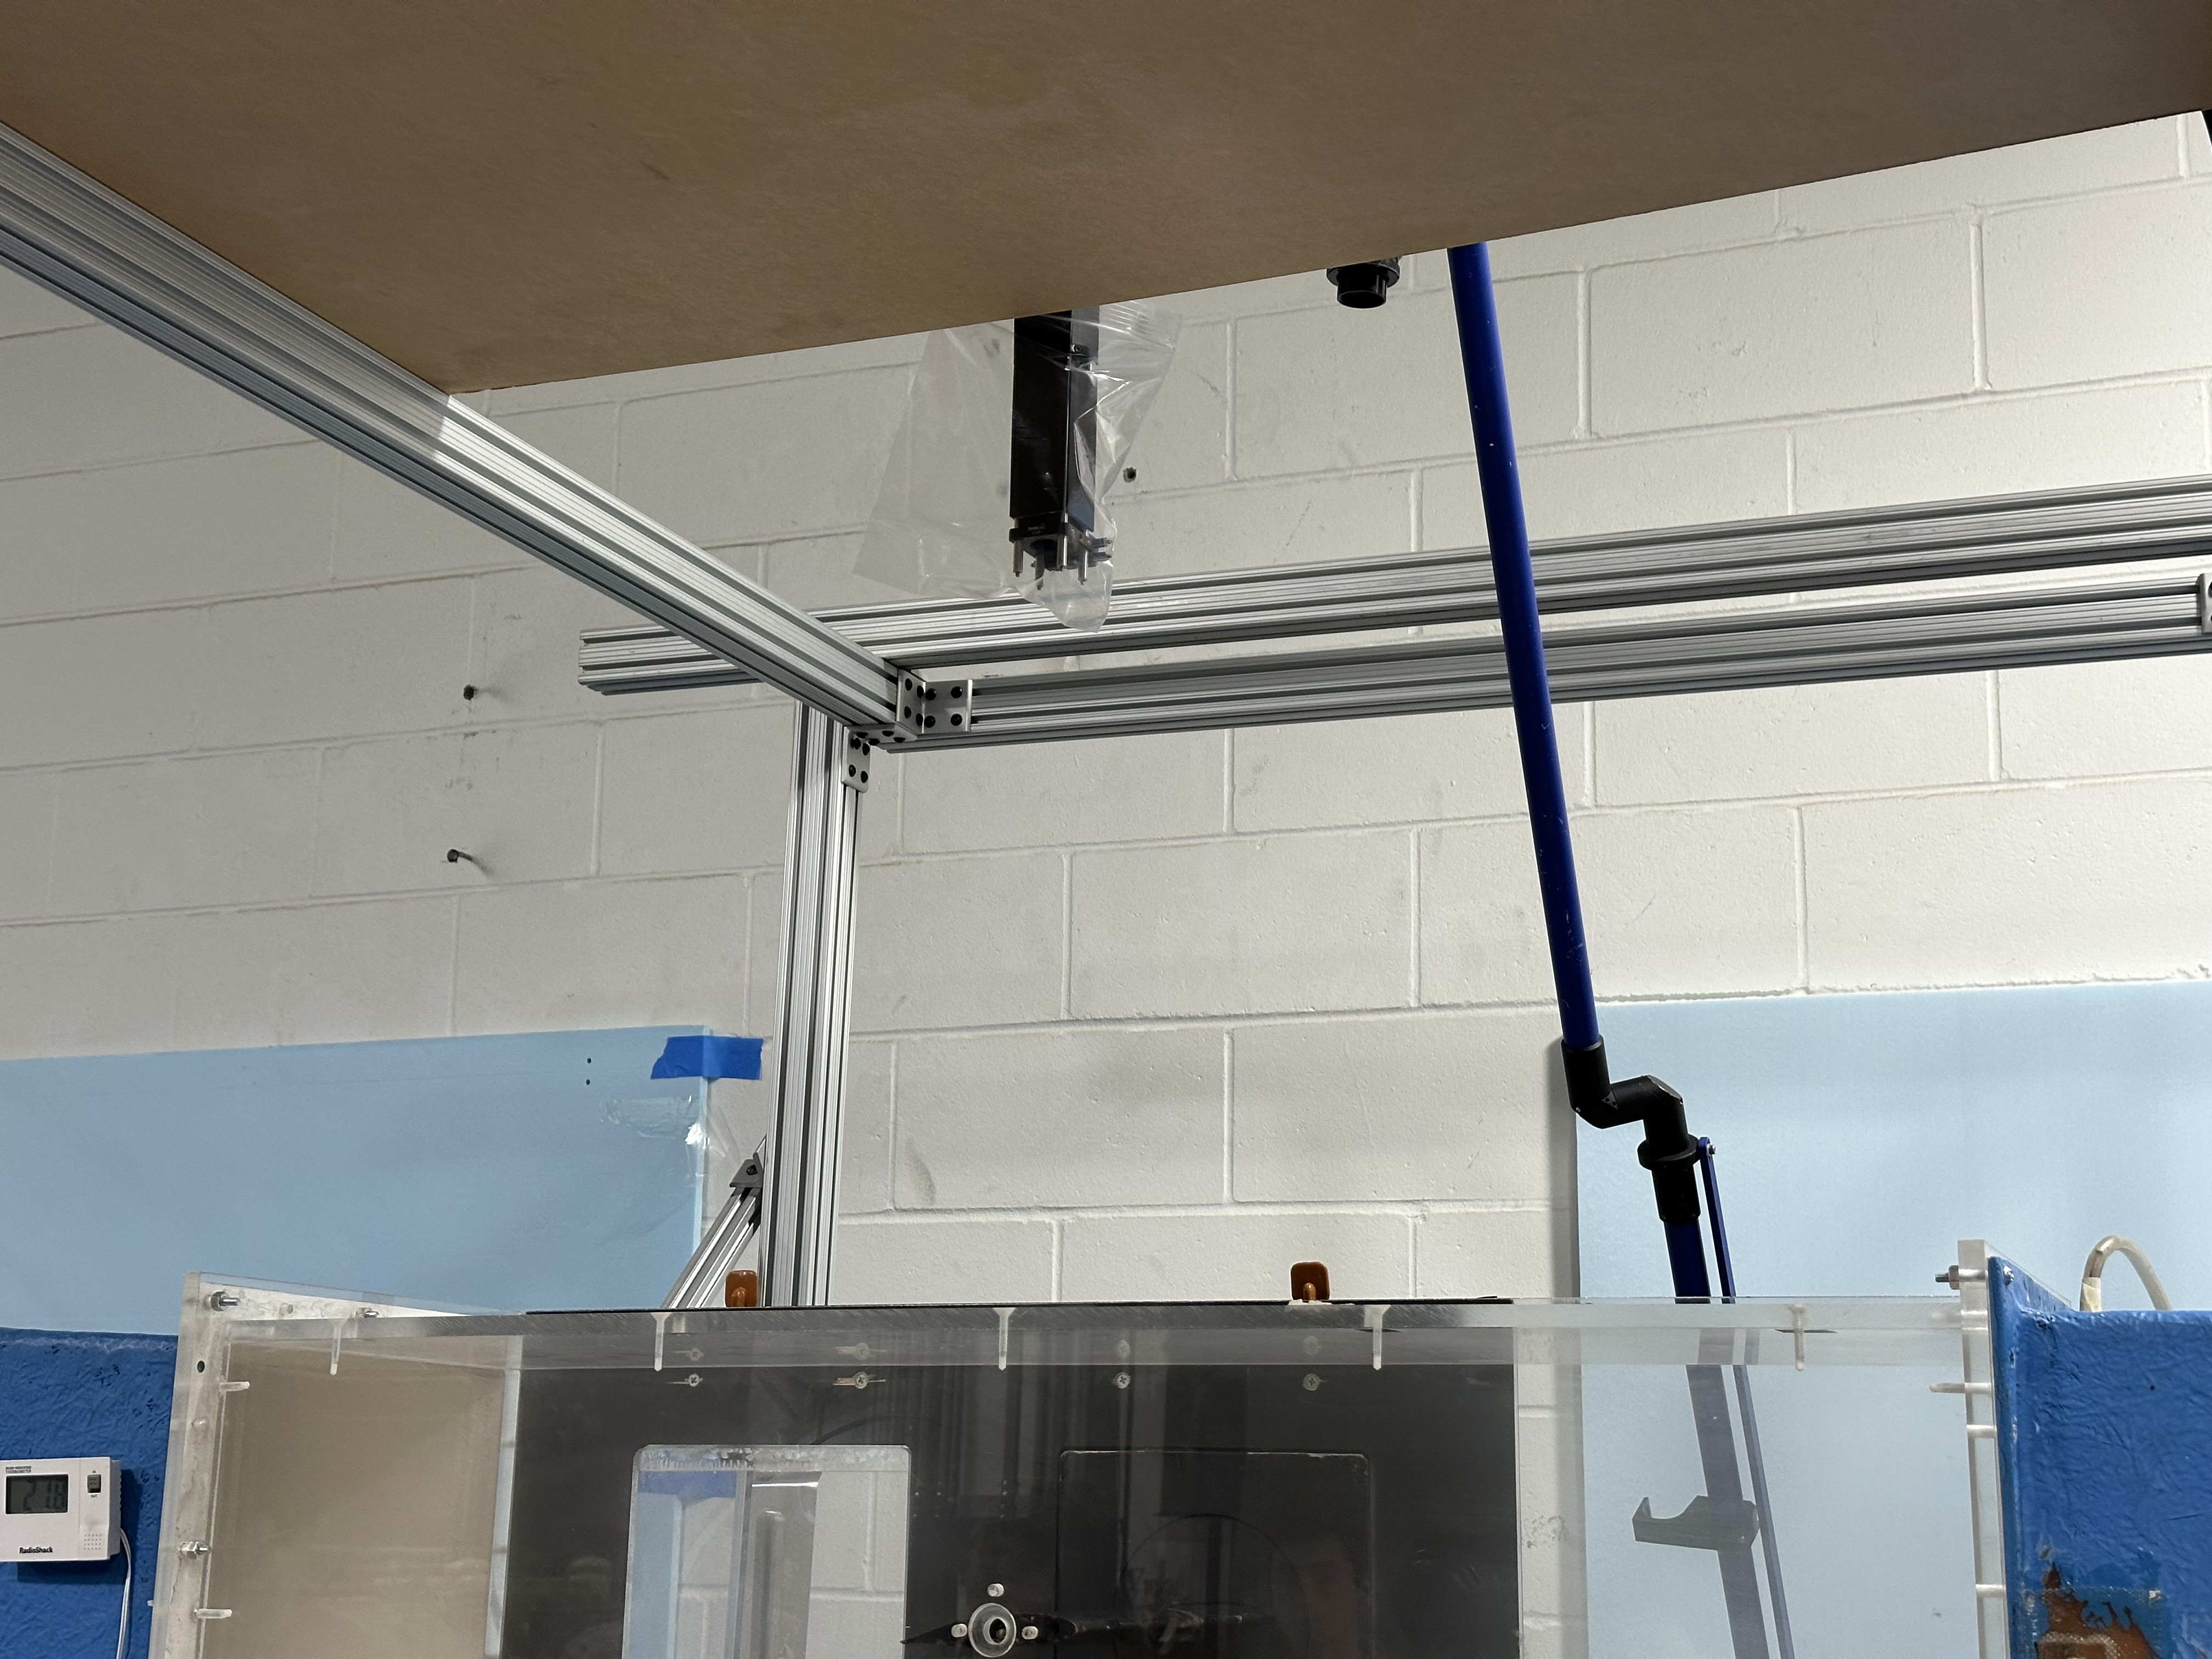
\includegraphics[width=\textwidth]{Figures/IMG_0130.jpeg}
        \caption{The laser used in \acrshort{piv} measurements.}
        \label{fig:laser}
    \end{subfigure} \\
    \begin{subfigure}{0.49\textwidth}
        \centering
        \includegraphics[width=\textwidth]{Figures/IMG_0129.jpeg}
        \caption{The high-speed camera used to capture \acrshort{piv} frames.}
        \label{fig:high-speed_camera}
    \end{subfigure}
    \begin{subfigure}{0.49\textwidth}
        \centering
        \includegraphics[width=\textwidth]{Figures/IMG_0131.jpeg}
        \caption{Frontal view of the \acrshort{piv} apparatus and the wind tunnel.}
        \label{fig:full_apparatus}
    \end{subfigure}
    \caption{Pictures of the apparatus.}
    \label{fig:apparatus}
    \vspace*{3.5in}
\end{figure}

\section{Procedure} \label{sec:Prodedure}

\begin{enumerate}
\item Set the wind tunnel to 10 $m/s$.
\item Set the \acrshort{aoa} to 4 degrees.
\item Set up the system as described in \autoref{sec:Apparatus}.
\item Start recording data using the data collection software.
\item Repeat steps 1-4 for 8, 12, and 16 degrees.
\end{enumerate}

\newpage

\section{Derivations} \label{sec: Derivations}

The PIV Data consists of x and y positions with corresponding x and y velocity. From the velocity data at each point, vorticity is found using \autoref{eq:vorticity}. This is computed using the \verb|curl| function in \acrfull{matlab} as the $k$ component of the velocity vector is zero and the result is the same.
\begin{equation}\label{eq:vorticity}
    \omega _z = \frac{\delta V}{\delta x} - \frac{\delta U}{\delta y}
\end{equation}
\begin{equation}\label{eq:curl}
    \Delta \times Velocity = \begin{bmatrix} i & j & k \\ \frac{\delta}{\delta x} & \frac{\delta}{\delta y} & \frac{\delta}{\delta z} \\ U & V & W \end{bmatrix} = \begin{bmatrix} i & j & k \\ \frac{\delta}{\delta x} & \frac{\delta}{\delta y} & 0 \\ U & V & 0 \end{bmatrix} = (0,0,\frac{\delta V}{\delta x} - \frac{\delta U}{\delta y})
\end{equation}
Data at every position over $N$ frames is averaged to get the mean velocity components in the x and y directions (\autoref{eq:mean_velocity}). 
\begin{equation}\label{eq:mean_velocity}
    U = \sum^N_{i=1} \frac{u_i}{N}, V = \sum^N_{i=1} \frac{v_i}{N} 
\end{equation}
From the mean velocities, the turbulent velocity fluctuations are computed at each position, $u_i$(\autoref{eq:fluctuation}).
\begin{equation}\label{eq:fluctuation}
    \overline{u}' = \sqrt{\sum^N_{i=1}(u_i-U)^2/N},
    \overline{v}' = \sqrt{\sum^N_{i=1}(v_i-U)^2/N}
\end{equation}
Finally, the turbulent velocity fluctuations are used to find the turbulent kinetic energy distribution, as shown in \autoref{eq:kinetic} \citep{lab11-manual}.
\begin{equation}\label{eq:kinetic}
    TKE = \frac{1}{2}\rho(\overline{u}'^2 + \overline{v}'^2)
\end{equation}

